\chapter{A Little Theory}
\label{ch:alittletheory}
% ##################################################################################################################
\hfill \textbf{Author:} Andreas Horni 

\begin{center} 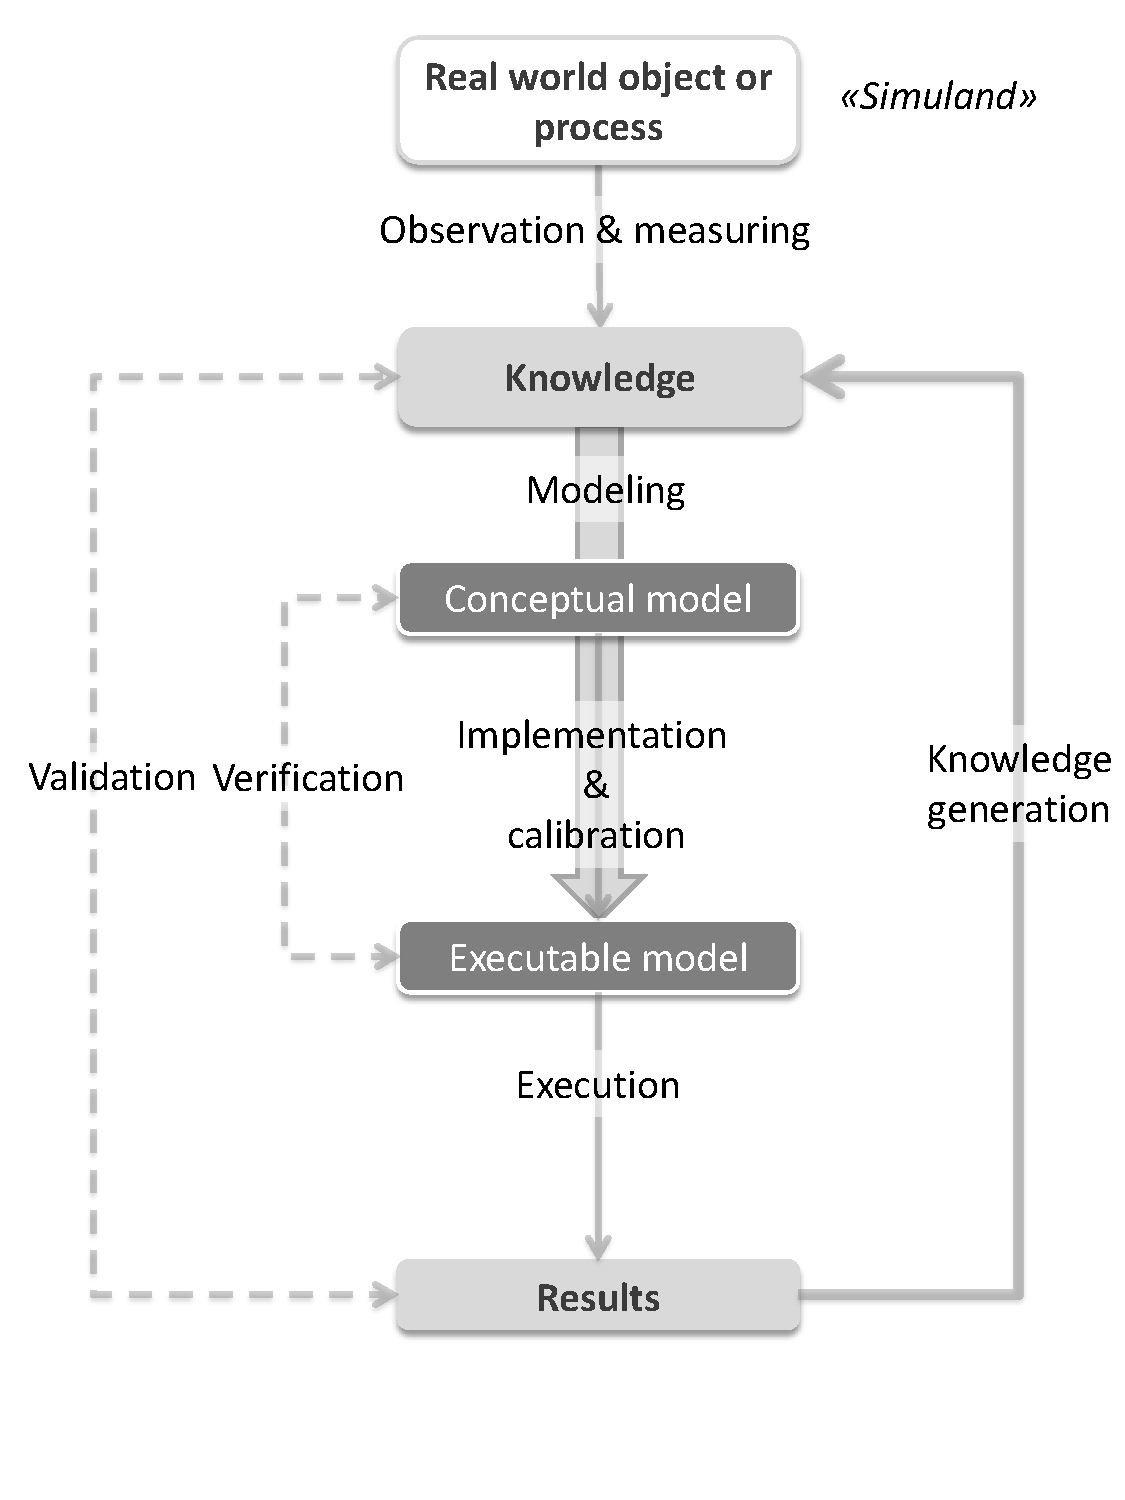
\includegraphics[width=0.4\textwidth, angle=0]{figures/modeling.pdf} \end{center}

% ##################################################################################################################
This chapters looks at theoretical aspects of transport planning and modeling (Sections \ref{sec:planning} and \ref{sec:transportmodeling}. Different strands of transport models are introduced with microsimulations in Section \ref{sec:transportmsims} as the central element of this book. 

\section{Transport Planning}
\label{sec:planning}
In societies based on the division of labor, production and consumption usually take place at different locations. Hence the relocation of persons, goods and messages, in other words transport---is essential generating benefits and costs not only for individual actors but also for the community. Due to its high significance the transport system requires planning where a main goal is the maximization of net benefit or social welfare through influencing the transport system spanning the infrastructure and its actors and in due consideration of the system's environment. Naturally, the definition of net benefit is highly complex and subject to societal discussion. Important questions are, among others, which factors require inclusion in the calculation or the weighting of individual and collective interests. Widely accepted criteria for guiding these political discussions are, e.g., \emph{Kaldor-Hicks efficiency} or \emph{Pareto efficiency}. But, the first first step for efficient control and understanding of transport system is transport modeling. 

% ##################################################################################################################
\section{Transport Modeling}
\label{sec:transportmodeling}
Before we look at the core of transport modeling in Section \ref{sec:equilibrium}, namely at the demand-supply paradigm and at the range of transport models in Section \ref{sec:models}, let us clarify the modeling basics and terminology.

In the strict system analysis perspective, three types of problems are distinguished, namely \emph{modeling} (or \emph{system identification}), \emph{optimization} and \emph{simulation} \citep[e.g.,][p.8ff]{EibenSmithJE_2003}. As shown in Figure \ref{fig:systemAnalysis} and described shortly below, for modeling problems (a) a model for known inputs and outputs is created, whereas for optimization problems (b) the model and some information about the output is known, and solving the problem means finding the input values. Simulations (c) produce outputs for known inputs and a given model. Often, particularly for complex problems, they co-exist and complement each other. 

Also in MATSim, all three problem types are present. \emph{Modeling} is done during MATSim model creation and calibration. The choice model parameters are estimated based on surveyed input and output data. \emph{Simulation} is applied in MATSim as infrastructure load simulation. \emph{Optimization} takes place, when individuals improve their individual day plan over the course of the iterations. % Categorizing the co-evolutionary algorithm adopted to compute the populations' Nash equilibria, however, is difficult.

% ----------
\createfigure%
{Problem categories of system analysis}%
{Problem categories of system analysis}%
{\label{fig:systemAnalysis}}%
{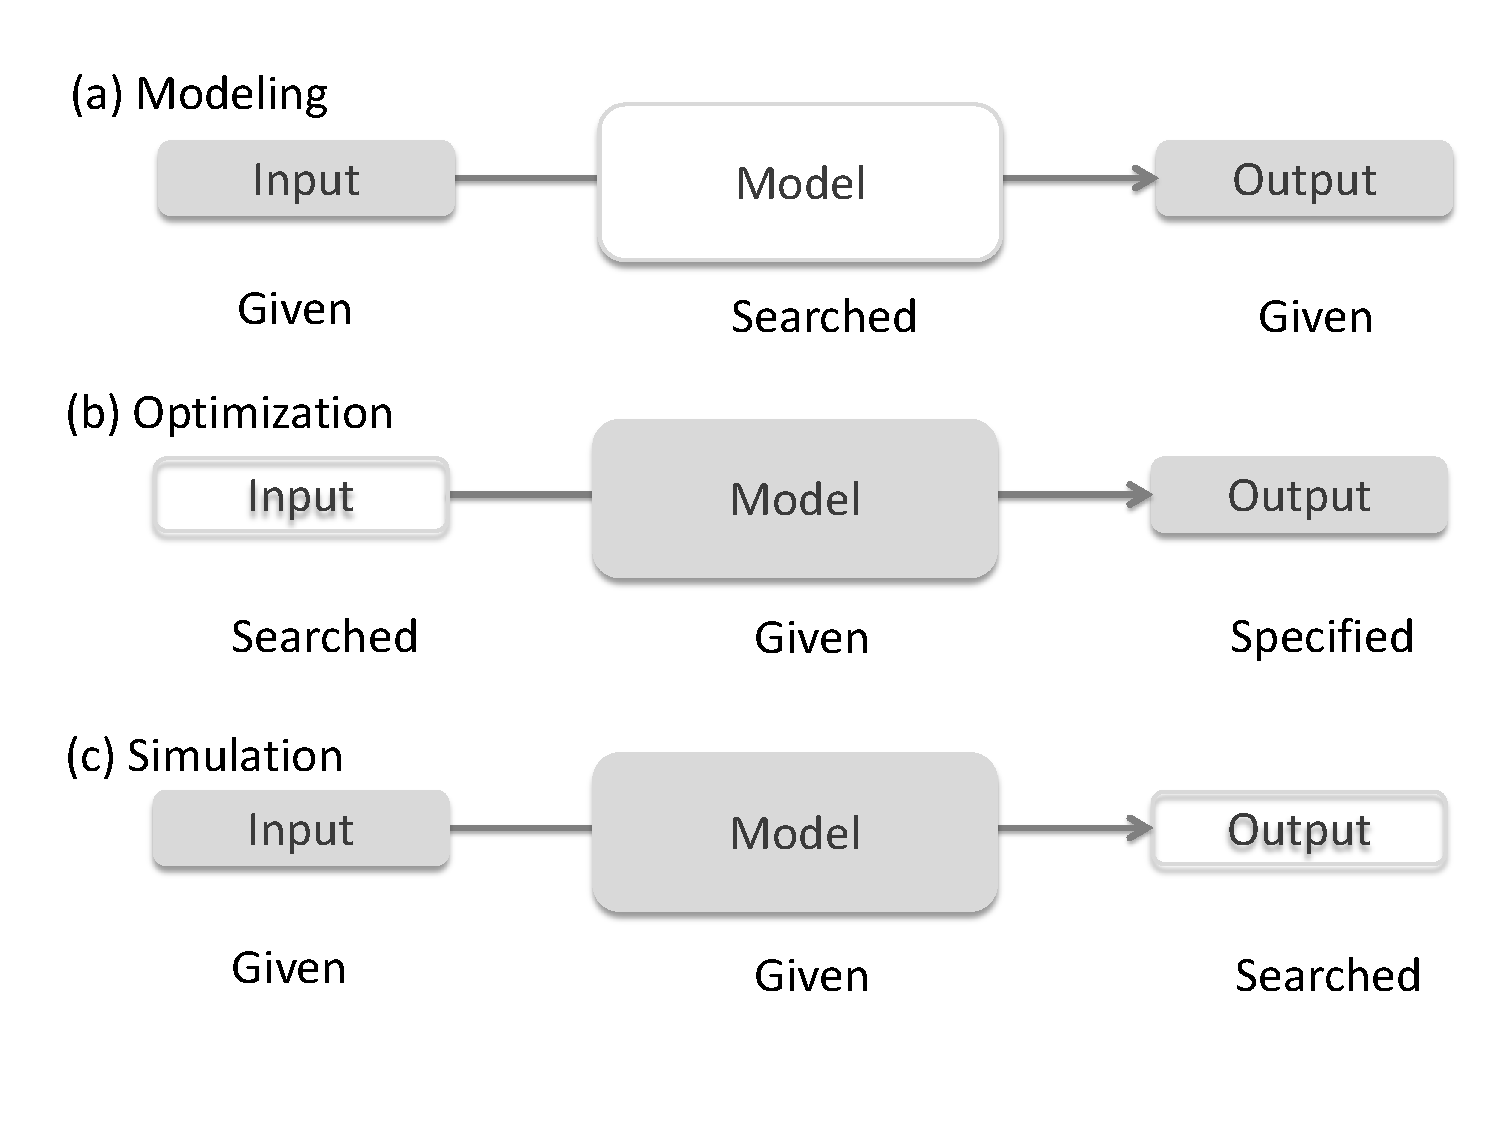
\includegraphics[width=0.8\textwidth, angle=0]{figures/systemAnalysis.pdf}}%
{}

% ----------

% ==========================================================================================
\subsection{Modeling}
\label{sec:alittletheory_modeling}
The term modeling is generally used in a in a more comprehensive sense than sketched above, actually, modeling is a universal and basically omnipresent and inevitable process while acting in this world. Already perception, creates an abstraction of reality, in philosophical terms, a simulacrum, and in more practical terms, a \emph{model}. 

In scientific contexts, the modeling enterprise looks as shown in Figure \ref{fig:modeling} loosely based on \citet[][Figure 10.2]{Petty_SokolowskiBanks_2010}. Modeling starts with observation and measurement of reality (in \citet[][]{Petty_SokolowskiBanks_2010} called ``\emph{simuland}'') for acquisition of knowledge (in \citet[][]{Petty_SokolowskiBanks_2010} called ``\emph{referent}''). Model creation, based on the modeler's knowledge about the world, is the core of the process at many places referred to as the actual \emph{modeling} step. Based on a conceptual model, an executable model is implemented and calibrated. The executable model is evaluated in a verification step in terms of ``\emph{was the model made right?}'' \citet[][p.332]{Petty_SokolowskiBanks_2010}. Validation compares results with the referent in the sense of ``\emph{was the right model made?}'' \citet[][p.332]{Petty_SokolowskiBanks_2010}. Calibration, verification and validation is detailed in Chapter \ref{ch:cvv}.
%
% -----------------
\createfigure%
{Modeling process}%
{Modeling process}%
{\label{fig:modeling}}%
{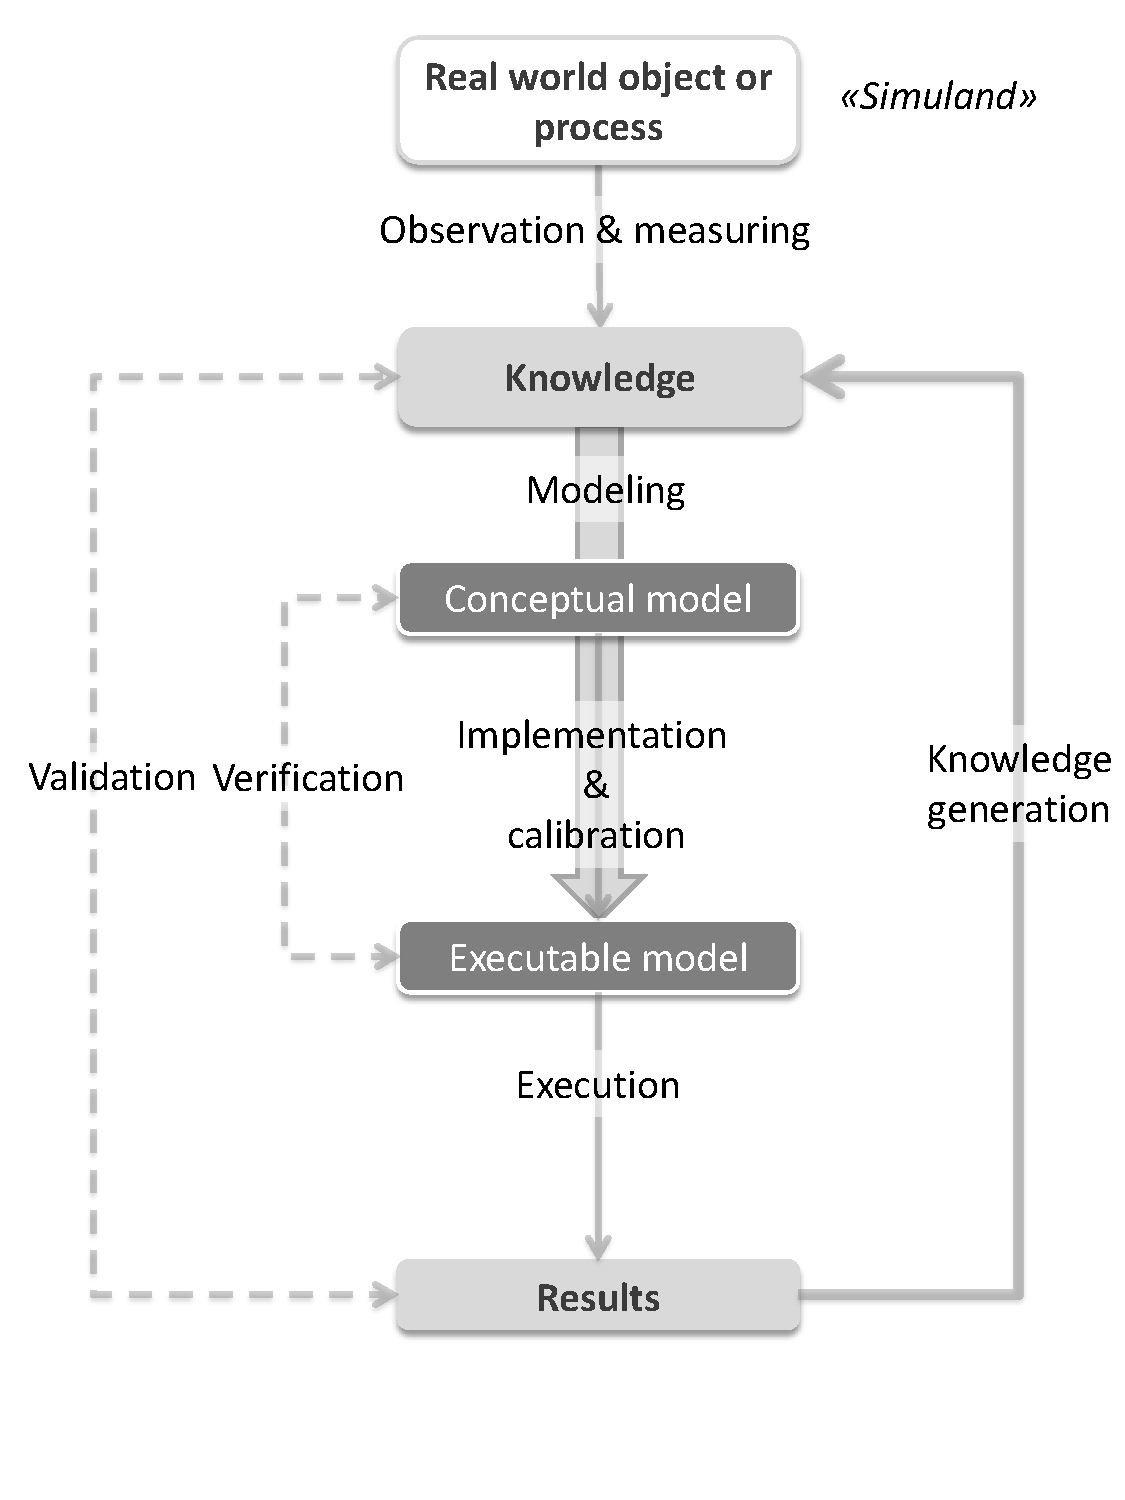
\includegraphics[width=0.8\textwidth,angle=0]{figures/modeling.pdf}}%
{}

% -----------------
%
\citet[][Section 1.9]{Epstein_Jass_2008} lists 16 reasons for modeling, of which in our opinion prediction, understanding, and experimentation are central. Strictly speaking, the final purpose of modeling is knowledge generation, shown on the right of Figure \ref{fig:modeling}, and often forgotten in similar depictions. The crucial question is ``\emph{can the model surprise us in a reasonable way?}'', as Eric Miller \footnote{professor at the university of Toronto.} asked the examinee in a PhD defense. A model that cannot surprise the modeler, i.e., increase the knowledge, is of little use. Due to the overwhelming complexity of simuland and the newness of the microsimulation approach, many microsimulation studies make progress in a verification rather than a validation perspective. In other words, modelers are often already satisfied, if models can be told something rather than modelers being told something by the model.

Finally, another important requirement for modeling is generalization. Robert Herman, as cited by \citet[][]{Mahmassani_Transportation_1988}, asks for more generalization and abstraction in transport planning: \begin{spacing}{1.0} ``\emph{We may not have had Ohm's law if Ohm was overly concerned with the detailed paths of the electrons and what these electrons were doing before crossing the resistor.}'' \end{spacing}

\ah{Create deep links from the different MATSim modeling stages) to this Section here}

% ==========================================================================================
\subsection{Demand-Supply Equilibrium Paradigm}
\label{sec:equilibrium}
The dominant paradigm of transport modeling, and the basis of MATSim, is the demand-supply equilibrium paradigm derived from a general economic perspective  \citep[][p.38]{BoyceWilliams_ERSA_2003}, \citep[][]{Bates_HensherButton_2000, Patriksson_1994}, \citep[][p.7]{OrtuzarWillumsen_2001}. The equilibrium assumption can be formulated as follows (see also e.g., \citet[][p.7f]{OrtuzarWillumsen_2001}. Transport infrastructure, interpreted as the supply side, provides a service, whose usage costs increase with demand, e.g., travel time is higher for higher loads. Under the reasonable assumption that demand is dependent on these costs, naturally, formation of a demand-supply equilibrium can be expected. Specific transport decisions are usually made by actors (e.g., travelers) optimizing \emph{their individual} benefit, thus, the equilibrium described above is termed \emph{user equilibrium}, reflecting Wardrop's first principle \citep[][]{Wardrop_PICE_1952, CorreaStier_Cochran_2010}. The efficiency of this descriptive state can be compared to the normative \emph{system optimum}, described by Wardrop's second principle. 

Clearly, this paradigm offers a parsimonious and elegant assumption but it is an approximation to reality and thus over time several differentiations concerning stochastic and dynamic aspects have been added (Section \ref{sec:types}). Furthermore, open questions about existence, uniqueness, stability and behavioral basis of equilibria exist, some of them raising serious doubts about its usefulness (Section \ref{sec:equiCharacteristics}).

% ---------------------------------------------------------------------------------------
\subsubsection{Types of Equilibria}
\label{sec:types}
% ------------------------------------------------------------------
Transport infrastructure is not static and, at least from modeler's perspective, also not deterministic. Extension of user equilibrium (UE) by randomness and dynamics leads to stochastic user equilibrium (SUE) and dynamic user equilibrium (DUE), respectively. Although, conceptually, this spans all choice dimensions, in early models, not all dimensions were included. Often, only route and time choice are subject to equilibration while mode, destination and activity chain choice are exogenous to models. Reasons are mostly of practical nature; models simply cannot be comprehensive from their beginnings.

Costs are usually given as \emph{generalized costs}. Traditionally, they are composed of individual time and money expenditures \citep[][p.12]{Bates_HensherButton_2000}, where, clearly, many further components exist. Externalities, i.e., not considered costs for non-users, such as immissions, become ever more important, hence, modern models should also be able to compute cases, where users monetarily compensate these external costs, in other words, where these costs are internalized.

% ------------------------------------------------------------------
\textbf{Deterministic User Equilibrium (UE):}
Deterministic user equilibrium is formulated by Wardrop's famous first principle \citet[][]{Wardrop_PICE_1952} as: \begin{spacing}{1.0} "\emph{The journey times on all routes actually used are equal, and less than those which would be experienced by a single vehicle on any unused route.}" \end{spacing}

According to \citet[][p.162]{BoyceEtAl_JRS_1988}, the first-known statement of user equilibrium dates back to \citet[][]{Pigou_1920} and was also discussed in \citet[][]{Knight_QJE_1924}. A rigorous mathematical formulation of user equilibrium is given in the seminal book of \citet[][]{BeckmannEtAl_1956}. Their optimization problem formalization made possible efficient algorithms for computation of user equilibrium, but this was not recognized immediately by transport modelers \citep[][p.26]{BoyceWilliams_ERSA_2003}. Surprisingly, the close relation to the Nash equilibrium \citep[][]{Nash_AM_1951, Nash_PNAS_1950} \footnote{
As succinctly put by \citet[][]{CorreaStier_Cochran_2010} "\emph{a Wardrop equilibrium can be viewed as an instance of a Nash equilibrium in a game with a large number of players"}.} was not mentioned by Wardrop but only nine years later by \citet[][]{CharnesCooper_Herman_1961}.

% ------------------------------------------------------------------
\textbf{Stochastic User Equilibrium (SUE):}
Clearly, travelers are \emph{not} perfectly informed, and from modelers' perspective some behavior looks stochastic, generating \emph{unobserved heterogeneity} in the surveyed data. These effects can be taken into account in the model by adding random error terms to the users perception, where, still each traveler is assumed to minimize his individual \emph{perceived} travel costs \citep[][p. 363]{OrtuzarWillumsen_2001} leading to stochastic user equilibrium \citep[][]{DaganzoSheffi_TransScience_1977}.  

% ------------------------------------------------------------------
\textbf{Dynamic User Equilibrium (DUE):}
Traffic is highly dynamic. One approach to take this into account and thus to increase model resolution, is to build independent time slices, for example for peak and non-peak hours, and to assume a static equilibrium for each of these periods. A more elegant approach is extension of the equilibrium formulation as follows. Conceptually, the user equilibrium can be made dynamic relatively straight forward. Instead of only taking into account route choice, departure time choice can be included. This means that no user can improve his performance by unilaterally changing his route or departure time \citep[see e.g.,][p.411]{Friesz_Hillier_2010}. Despite the conceptual straightforwardness, implementation of dynamic equilibrium models is complex.

% ------------------------------------------------------------------
\subsection{Existence, Uniqueness, Stability and Behavioral Basis of Equilibria}
\label{sec:equiCharacteristics}
For the design of algorithms to compute equilibria and the interpretation of their results, knowledge about the qualitative characteristics of the targeted equilibrium---such as existence, uniqueness and stability---usually are productive. Hence, these characteristics of aforementioned equilibriums have been researched intensively, \citet[][]{Dafermos_TransScience_1971, Smith_TransResB_1979, Smith_TransResB_1983} for the UE, \citet[][]{Daganzo_TransScience_1983} for the SUE and \citet[][]{Smith_TransResB_1993} for the DUE, to name only a few.

An essential component of an equilibrium formulation is its temporal and spatial domain. Equilibria, and its qualitative characteristics, can be local and global as well as short-term and long-term \citep[][p.8]{OrtuzarWillumsen_2001}. Furthermore, equilibrium can span multiple dimensions, including destination and activity type choice. This leads to day plan equilibria, which are \emph{not} necessarily in equilibrium for every single choice dimension considered in isolation. A day plan equilibrium, for example, does not necessarily include a Wardrop equilibrium, if, in some situation, further driving generates a higher utility than waiting at the destination, while paying parking costs \footnote{Peter Vovsha, personal communication, July 2012}. %\ah{Vovsha, Madison -> Kenneth Small, Parking costs!}

Clearly, the concept of equilibrium, in particular the UE, is an abstraction from, and thus, an approximation to reality and it is discussed controversially \citep[see e.g.,][p.58ff]{Patriksson_1994}. The fundamental question concerns existence of equilibria in reality and their evolution from non-equilibrium states \citep[][p.254]{PeetaZiliaskopoulos_NSE_2001}. \citet[][]{Horowitz_TransResB_1984}, for example, investigated a simple 2-link network in terms of SUE and did not find dominating stability. He concludes that \emph{``the validity of the standard assumption about the achievement of equilibrium appears to be highly questionable''}. \citet[][p.251]{Holden_JTEP_1989}, in a theoretical paper, criticizes UE assumption in context of a potentially chaotic system and in absence of a stringent behavioral basis. On the other hand, \citet[][]{FrieszEtAl_OpRes_1994}, later, investigated day-to-day adjustment processes toward a static Wardrop user equilibrium, and demonstrated that, eventually, an equilibrium state is reached. \citet{Mahmassani_unpub_WCTR_1989} empirically found the same in laboratory experiments.

Sometimes also intuition is in conflict with the equilibrium notion. The Braess paradox \citep[][]{Braess_UF_1969} and the (Pigou-Knight-)Downs(-Thompson) paradox \citep[e.g.,][]{Downs_TQLY_1962} describe how adding supply can, counter-intuitively, increase usage costs require caution in application of the equilibrium paradigm.

For microsimulations---usually being highly dynamic, stochastic and disaggregate with many user classes and behaviorally rich decision principles---unfortunately very little is known about the targeted equilibria.

% ==========================================================================================
\subsection{Models}
\label{sec:models}
% -----------------------------------------------------------------------------------
\subsubsection{The 4-Step Procedure}
Still the main method in transport planning practice and the basic structure of most modern executable planning models (see Figure \ref{fig:g12Models}) is the 4-step procedure also known as urban transportation planning procedure (UTP) \citep[][p.17ff]{Bates_HensherButton_2000}, \citep[][p.2]{CFD_TRB_2007}, \citep[][]{McNally_HensherButton_2000}. The 4-step procedure was developed in the 1950ies in the Detroit Area Transportation Study and Chicago Area Transportation Study (CATS). A very detailed history of transport models including its political dimension is presented by \citet[][]{Weiner_2008}. The UTP belongs to the aggregate, sometimes called first-generation methods \citep[][p.20ff]{OrtuzarWillumsen_2001}. In the classic model, the demand is assigned to the infrastructure by trip generation and attraction, trip distribution, mode choice and assignment. In the early implementations, feedback was only present within the assignment step but not between steps. \citet[][p.27]{BoyceWilliams_ERSA_2003} report on the problem of tenuous behavioral basis for the linking of the single steps. The UTP is an efficient and suitable approach for supporting the making of decisions relevant at the time of its invention, which was infrastructure extension \citep[][Section 2]{Kitamura_TMIP_1996} (``car was king'' \citep[][]{Daly_unpub_STRC_2013}). With the shift from extending to managing the infrastructure, disaggregate, also called second generation, models were proposed. 

% --------------
\createfigure%
{Comparison of first and second generation transport models}%
{Comparison of first and second generation transport models}%
{\label{fig:g12Models}}%
{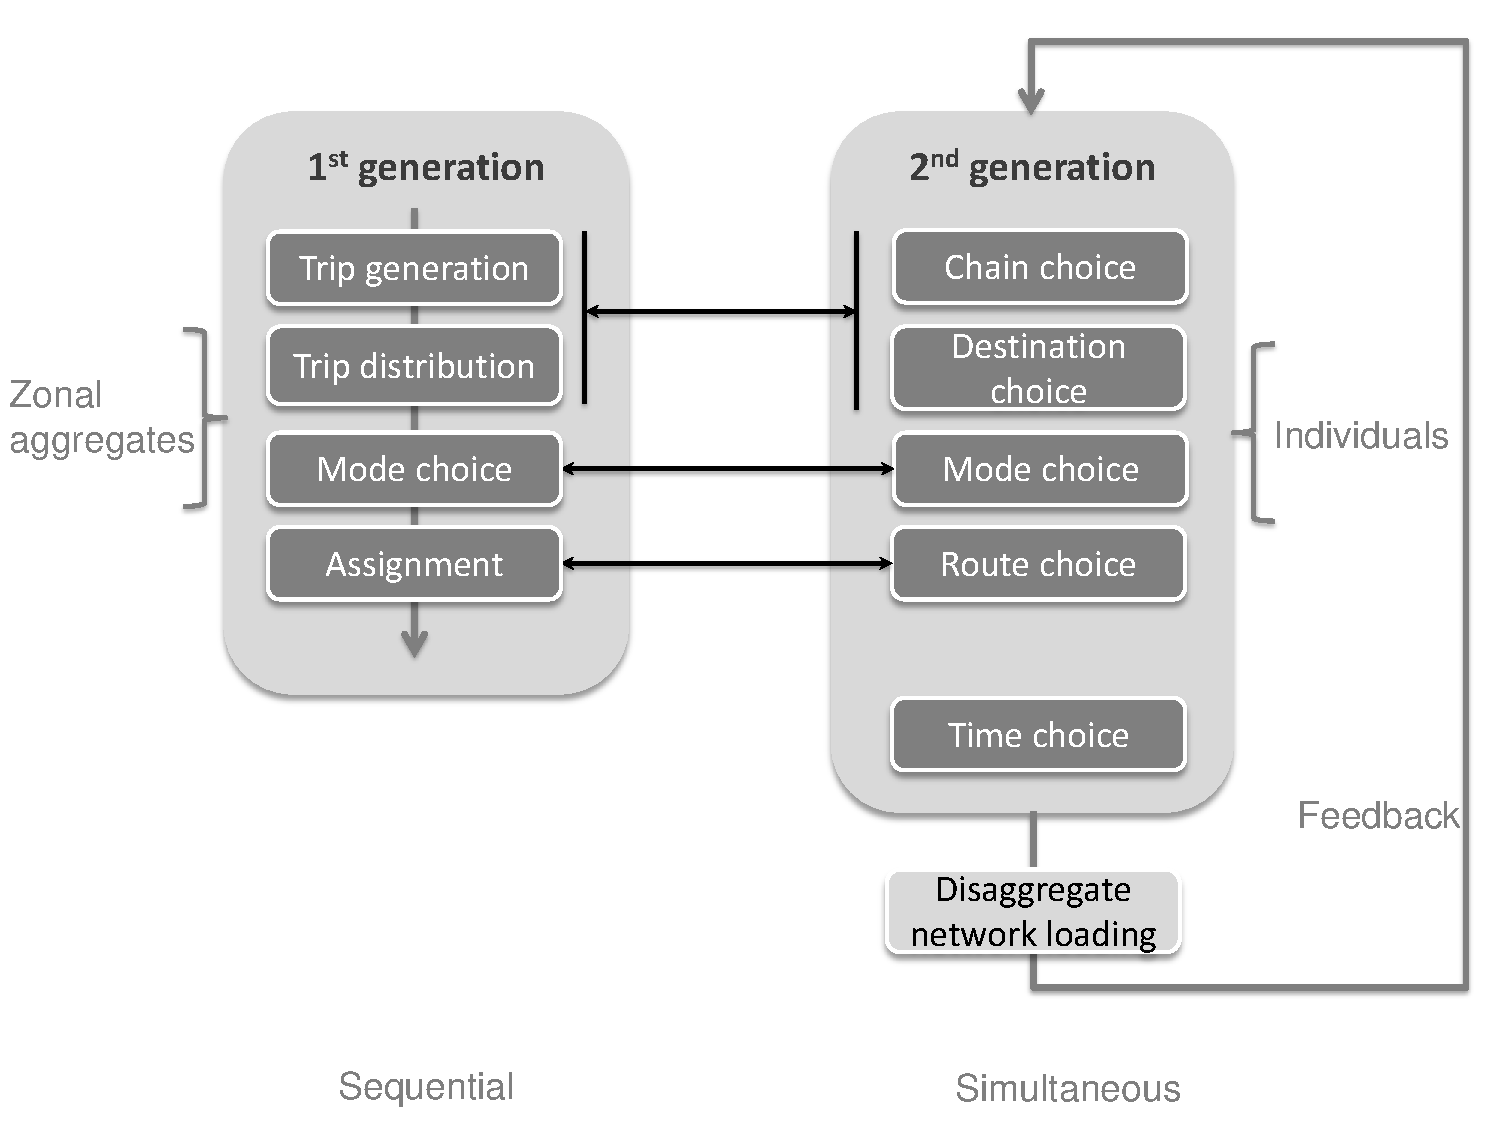
\includegraphics[width=0.99\textwidth, angle=0]{figures/g12Models.pdf}}%
{}

% --------------
% -----------------------------------------------------------------------------------
\subsubsection{Disaggregate Models and the Activity-Based Approach}
\citet[][Slide 4]{Bhat_unpub_1998} depicts the evolution of travel demand forecasting techniques, from aggregate trip-based to disaggregate trip-based approaches and then to the activity-based paradigm. ``Disaggregate'' means that the basic modeling unit is the individual (see e.g., \citet[][]{BenAkiva_TRR_1974, DomencichMcFadden_1975, BenAkivaLerman_1985}, \citet[][p.20]{OrtuzarWillumsen_2001}). The dominant paradigm of disaggregate modeling since the late 1970s is discrete choice modeling \citep[][p.30]{BoyceWilliams_ERSA_2003}. 

The improvements of the second generation models over first generation models, listed at many places (see e.g., \citet[][]{Axhausen_SSRL_2006}, \citep[][p.3]{SbaytiRoden_ResRep_AASHTO_2010}, \citet[][Section 2.2]{McNallyRindt_TechRep_UCI_2008}, \citep[][]{BhatKoppelman_HallRW_2003, CFD_TRB_2007}), can be summarized as follows:

\begin{spacing}{1.0}
\begin{itemize}
	\item \emph{Individual persons instead of zonal aggregates:} This allows to directly and naturally apply the choice models for all dimensions at the individual level, not requiring aggregation, potentially making the behavioral basis stronger.
	\item \emph{Activity chains instead of single independent trips, considering trip chaining} 
	\item \emph{Applying Feedback:} In the basic first generation models, feedback only appears in the fourth stage (e.g., in the method of successive averages). Although some improved models of the first generation already contain feedback of the network conditions to earlier stages, essentially the feedback, spanning the complete process is a feature of the second generation models. Clearly, taking into account feedback strongly improves the results quality.
	\item \emph{Simultaneous choice instead of sequential procedure}
	\item \emph{Higher temporal resolution:} Basically the first generation models are static. Some dynamics have been added (e.g., hourly origin-destination matrices) in later models. Nevertheless, this is always associated to usually quite large and fixed time steps. Explicitly including the time choice dimension, as in second generation models, promises a much higher temporal resolution, where, even though the \emph{results} are usually again given as hourly aggregates, the results quality is expected to be higher if aggregation is done at the very end of the modeling.
	\item \emph{Schedule equilibrium instead of Wardrop equilibrium:} If further dimensions than only route choice are taken into account while searching for a user equilibrium, this equilibrium is not necessarily associated to a Wardrop equilibrium (i.e., network equilibrium). Also, the existence and the uniqueness of a user equilibrium is not assured anymore. However, targeting at a planning equilibrium is behaviorally more sound.
\end{itemize}
\end{spacing}

The most prominent instance and extension of disaggregate modeling are activity-based models. They are based on the fundamental principle that ``\emph{travel demand is derived from activity demand}'' \citep[][]{Jones_HensherStopher_1979, Bowman_TEC_2009_1, Bowman_TEC_2009_2, BhatKoppelman_HallRW_2003, EttemaTimmermans_1997, BowmanBenAkiva_ABTFCEngelke_1996, BowmanBenAkiva_TransResA_2001}. 

The roots of this approach are wide-spread. The literature names multiple seminal papers as roots of the activity-based analysis, such as \citet[][]{Haegerstrand_PRSA_1970, Chapin_1974, FriedEtAl_ResRep_NCHRP_1977} or \citet[][]{Kreibich_Transportation_1979} (published in Germany in 1972), cited in \citet[][]{AxhausenHerz_JTE_1989} and by \citet[][p.165]{Miller_ABTFC_1996}. \citet[][Section 3]{McNallyRindt_TechRep_UCI_2008} see the linkage of activity and travel participation established already by \citet[][]{MitchellRapkin_1954}. Despite these numerous early papers, it took very long until operational models were available \citep[][p.31]{BoyceWilliams_ERSA_2003}. \citet[][Figure 2]{Bowman_TEC_2009_1} provides a timeline of US activity-based implementations. Today, many microsimulations are implemented within the activity-based framework.

% ---------------------------------------------------------------------------------------
\subsubsection{Assignment Methods: Successors of Beckmann et al.}
For traffic assignment, non-equilibrium \citep[][]{Matsoukis_TPT_1986} and equilibrium methods \citep[][]{MatsoukisMichalopoulos_TPT_1986, Patriksson_1994} exist. A major equilibrium algorithm to solve the static assignment problem is the ``Method of Successive Averages'' (MSA) rooted on \citet[][]{RobbinsMonro_AMS_1951} and \citet[][]{Blum_AMS_1954} \footnote{
A clarification of the intricate adoption of the MSA in transport modeling is currently undertaken by \citet[][]{BoyceWilliams_forthcoming}, where relevant further information can also be found in \citet[][]{Smock_HRBB_1962, LeBlanc_PhDThesis_1973, Nguyen_TransScience_1974, LeBlancEtAl_TransRes_1975, VanVliet_BonsallEtAl_1977, SheffiPowell_TransResB_1981}).
}. An important issue for the MSA is the re-assignemnt share of link flows, where reaching a Nash equilibrium is guaranteed by decreasing the re-assignemnt share \citep[see, e.g.,][]{PowellSheffi_TransScience_1982, Sheffi_1985}). Efficiency of the algorithm can be improved by optimizing this share with the Frank-Wolfe algorithm \citep[][]{FrankWolfe_NRLQ_1956}.

Besides methods that search for the deterministic user equilibrium, procedures for performing stochastic traffic assignment \citet[see e.g.,][]{Dial_TransRes_1971, SheffiPowell_TransResB_1981, Willumsen_HensherButton_2000, CorreaStier_Cochran_2010}, and dynamic traffic assignment \citep[][]{PeetaZiliaskopoulos_NSE_2001, LinDYEtAl_TRR_2008, ChiuEtAl_TechRep_TRB_2010, FrieszBernstein_HensherButton_2000} were developed.

Besides a plethora of practice models based on the 4-step procedure, there is a strand of mathematical models relatively slowly entering practical models. They can be called the successors of \citet[][]{BeckmannEtAl_1956} as they apply relatively complex mathematical techniques for computation and qualitative analysis of equilibria, where mathematical programming, optimal control, and variational inequality formulations are dominating \citep[][]{KinderlehrerStampacchia_1980, Dafermos_TransScience_1980, Smith_TransResB_1979, Dafermos_MP_1983, Smith_TransResB_1993, FrieszEtAl_OR_1993, Smith_TransResB_1993, Nagurney_1993, Friesz_TransScience_1996, Nagurney_FloudasPardalos_2001, BierlaireCrittin_TransScience_2006, LinDYEtAl_TRR_2008, Friesz_Hillier_2010, HarkerPang_MP_1990, NoorEtAl_JCAM_1993}. An interesting framework, combining the advantages of both dynamical systems \citep[e.g.,][]{Jin_TransResB_2005} and variational inequalities, are projected dynamical systems, which are suitable for studying dynamic traffic assignment, and its non-equilibrium states \citep[][]{NagurneyZhang_1996, Nagurney_FloudasPardalos_2009, DupuisNagurney_AOR_1993}.

A substantial gap exists between these ``analytical'' approaches \citep[][p.234]{PeetaZiliaskopoulos_NSE_2001}, and simulation-based approaches in terms of equilibrium analysis. Although it may be very difficult if not impossible to specify large-scale microsimulation equilibria with specific mathematical terms such ``convex, finite, compact, coercive, continuous, montone'' etc., we nevertheless stick to \citet[][p.243]{PeetaZiliaskopoulos_NSE_2001} saying that \begin{spacing}{1.0} "\emph{[...] an ability to analyze the system properties even under simplified assumptions can be insightful in generating future directions to address problems}". \end{spacing}



% ##################################################################################################################
\section{Transport Microsimulations}
\label{sec:transportmsims}
Decomposing a system into its parts and investigating the isolated parts is the canonical paradigm in research. However, many systems elude analysis, in this strict meaning of the word. The interactions of the many system components, whether they are sand grains in an dune avalanche or drivers in a phantom jam, generate system properties being more than the sum of the single components and thus a different research approach needs to be adopted for these \emph{complex systems}. Stephen Hawking claims that ``complexity is the science of the 21st century''; actually, computers give research a tool at hand by which such systems and its emergent properties can be investigated adequately with a bottom-up approach: simulations, or to be more precise microsimulations, which model the temporal development of a real-world system or process by explicitly considering the interactions of micro units such as individuals or vehicles. For concise definitions and further information see e.g., \citet[][Section 2]{Miller_ABTFC_1996} or \citet[][p.3]{Banks_2001}, \citet[][]{Bossel_2004} or \citet[][]{Orcutt_RESQ_1957}, who is often referred to as the inventor of microsimulation.

According to above definition, only the program components that model transition processes should be termed microsimulation. Strictly speaking, in MATSim for example, only the network loading simulation is actually a simulation. However, the delineation is difficult and, thus, in the transport planning community, the term \emph{microsimulation} is ambiguously used. Sometimes it actually denotes only the simulation of traveling persons and vehicles in the assignment step---as a replacement of volume-delay functions in aggregate models \citep[see e.g.,][p.508]{NagelBarrett_IJMPC_1997}. More often, it additionally includes the preceding choice processes \citep[][]{Kitamura_TMIP_1996, LiuEtAl_TransResA_2006}. In this sense, microsimulation includes the activity-based demand modeling part and the dynamic traffic assignment (for a detailed discussion of combination of these two parts see \citet[][p.10ff]{Balmer_PhDThesis_2007}).

Microsimulations are a consistent implementation of the disaggregate paradigm and offer a variety of benefits as for example listed by \citet[][]{Miller_ABTFC_1996, VovshaEtAl_TRR_2002, NagelBarrett_IJMPC_1997, Bonabeau_PNAS_2002, CharyparEtAl_TRR_2007}. In our opinion, the most important ones are, first, the high precision in computing the network loading \citep[][p.508/524]{NagelBarrett_IJMPC_1997}, second, the reproduction of complex interactions (as occurring for example for parking traffic) and, thus, the appropriateness for capturing emergent phenomena \citep[][]{Bonabeau_PNAS_2002}, and, third, the conceptual consistency by using the individuals as simulation units throughout the complete modeling process. These microsimulation features meet the challenging set of requirements for transport modeling added by the the shift from infrastructure expansion, where ``\emph{car was king}'' \citep[][]{Daly_unpub_STRC_2013}, toward infrastructure management, experienced in many places over the recent years. These conceptual advantages, together with the large research body, the continuously increasing computational power, and a large availability of microsimulation software packages create the potential for microsimulations to become state-of-practice in efficiently complementing the aggregate approach.

Clearly, the high model resolution and sensitivity comes at a price. Microsimulations are highly demanding in terms of data, as, naturally, they need to have the equally high resolution. Large-scale microsimulation scenarios are thus associated to financial, privacy, but also methodological issues. Falling back to disaggregation procedures applied on aggregate data, such as \citet[][]{BalmerRieser_TechRep_IVT_2004}, naturally, strongly reduces the resolution. However, many correlations are still consistently captured in the day plans. The complexity of large-scale microsimulators requires a broad knowledge of the specific microsimulation interna for calibration, verification, validation, and finally application \citep[e.g.,][p.273]{SmithEtAl_JTE_2008}. Furthermore, with the currently given data base for large-scale scenarios, the conceptual advantages of microsimulations over traditional aggregate models are difficult to show \citep[][]{LempEtAl_TRR_2007}.

A common distinction of microsimulations is between equilibrium-based models and computational process models \citep[][]{Hunt_TRBTDF_2006, ArentzeEtAl_Hensher_2001}. As shown in Figure \ref{fig:statesAndTransitions}, the paradigms differ as follows. Computational process models concentrate on the transition process leading from a reasonable starting situation to an essentially unknown outcome or end situation. This transition process is thereby made as behaviorally sound as possible. Equilibrium-based models claim to know the structure of the outcome, namely a demand-supply equilibrium. Start point and transition process, or in this case equilibration process, are only relevant in terms of efficiency but not with regard to content. Consequently, equilibrium models are inherently iterative, where computational process models are based on sequential procedures. For adequate handling of randomness, both paradigms need to be based on ensemble runs. 
%
% -------------------
\createfigure%
{Comparison of equilibrium and computational process models}%
{Comparison of equilibrium and computational process models (bounded rationality)}%
{\label{fig:statesAndTransitions}}%
{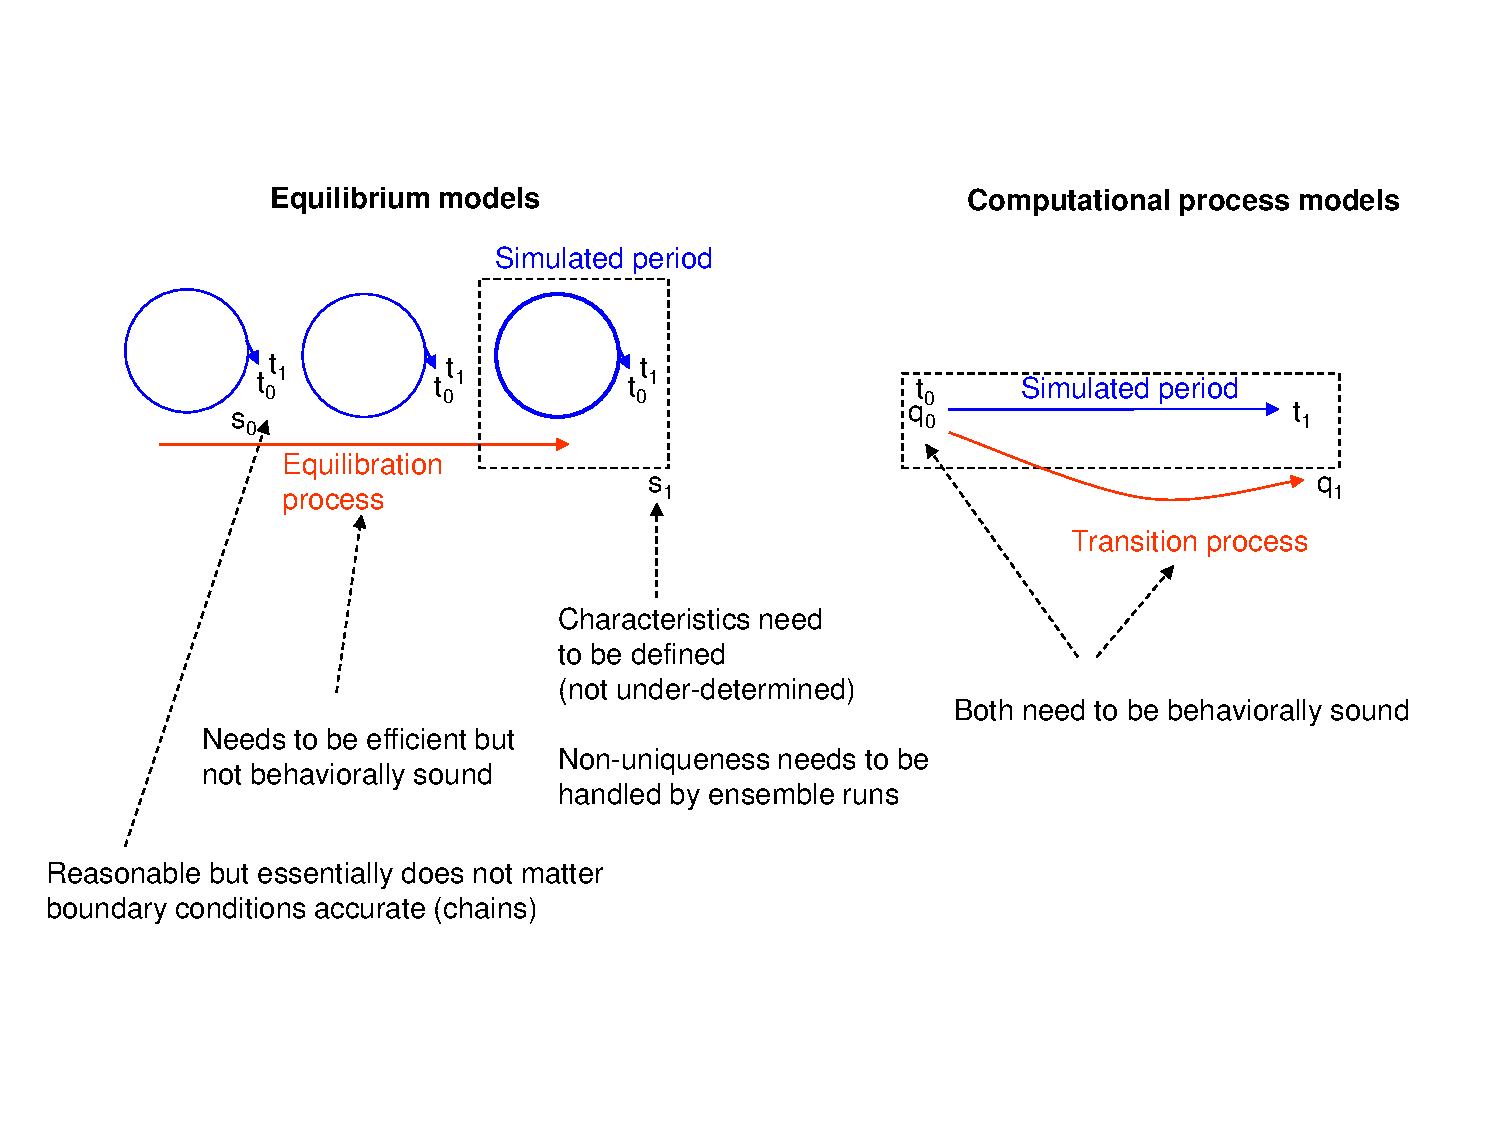
\includegraphics[width=1.3\textwidth,angle=90]{figures/StatesAndTransitions.pdf}}%
{}

% -------------------
\ah{
Rule-based versus equi-based \\

Fit observations: \\
Equilibirum models: add $\epsilon$s \\
Rule-based models: add more rules \\

top-down versus bottom-up? \\

equilibrium models: rule-based model with only one rule? \\
}


Microsimulations come at different levels of detail, lying between mesoscopic and submicroscopic simulations and ranging from complex car following models to cellular automaton to efficient but relatively rough queue-based models (as used in \citet[][]{Gawron_IJMPC_1998}) (for detailed reviews on traffic flow models see also \citet[][]{HoogendoornBovy_PImechE_2001}, \citet[][]{DarbhaEtAl_NA_2008}). In MATSim, a queue-based, event-based mobility simulation is employed per default \citep[][]{CharyparEtAl_TRR_2007}.

Various microsimulations, among them MATSim, adopt the multi-agent approach \citep[p.172ff][]{GilbertTroitzschKG_2005}, \citep[][]{Bonabeau_HBR_2002, SanfordBernhardt_TRBC_2007, Sun_2006}, being a subfield in artificial intelligence research. In the words of \citet[][p.7280]{Bonabeau_PNAS_2002} agent-based modeling is the ``\emph{canonical approach to modeling emergent phenomena [...]}''. An agent according to \citet[][p.21]{Wooldridge_2009} \begin{spacing}{1.0} ``\emph{is a computer system that is situated in some environment, and that is capable of autonomous action in this environment in order to meet its delegated objectives.}''. \end{spacing}

% ##################################################################################################################